\documentclass[border=10pt]{standalone}
\usepackage{tikz}
\usetikzlibrary{calc}

\begin{document}

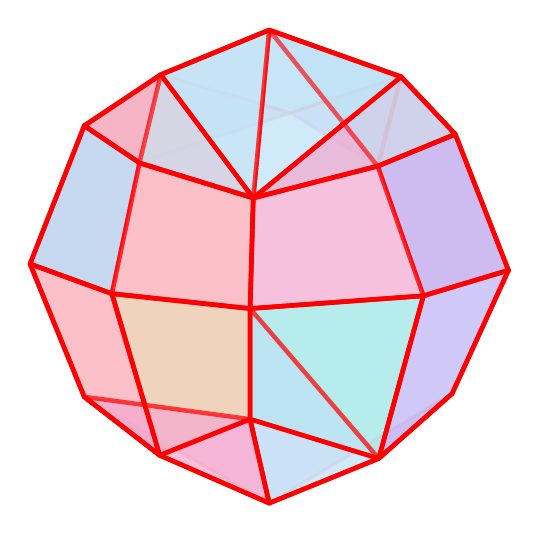
\begin{tikzpicture}[scale=1.35, line join=round, line cap=round, every node/.style={transform shape}]
  % Pastel face colors used across the kite faces
  \definecolor{faceBlue}{RGB}{150,205,238}
  \definecolor{faceBrown}{RGB}{229,184,150}
  \definecolor{faceGreen}{RGB}{155,226,204}
  \definecolor{faceViolet}{RGB}{165,150,238}
  \definecolor{faceMagenta}{RGB}{238,135,188}
  \definecolor{faceCyan}{RGB}{139,225,225}
  \definecolor{faceOrange}{RGB}{248,184,132}
  \definecolor{faceRed}{RGB}{248,132,150}
  \definecolor{faceLavender}{RGB}{190,170,235}
  \definecolor{faceSky}{RGB}{165,215,242}

  % Upright projected vertices of a compact deltoidal icositetrahedron
  \coordinate (T)  at (0.00, 2.20);
  \coordinate (UL) at (-1.02, 1.78);
  \coordinate (UR) at (1.24, 1.76);
  \coordinate (OL) at (-1.74, 1.30);
  \coordinate (OR) at (1.75, 1.22);
  \coordinate (L)  at (-2.25, 0.00);
  \coordinate (R)  at (2.25, -0.06);
  \coordinate (LL) at (-1.74,-1.25);
  \coordinate (LR) at (1.72,-1.22);
  \coordinate (BL) at (-1.03,-1.80);
  \coordinate (BR) at (1.03,-1.83);
  \coordinate (B)  at (0.00,-2.25);

  \coordinate (A)  at (-1.22, 0.95);
  \coordinate (C)  at (1.02, 0.92);
  \coordinate (M)  at (-0.15, 0.62);
  \coordinate (N)  at (0.20, 1.42);
  \coordinate (P)  at (-1.48,-0.28);
  \coordinate (Q)  at (1.45,-0.30);
  \coordinate (S)  at (-0.18,-0.42);
  \coordinate (U)  at (-0.18,-1.46);

  % Back/overlapping translucent kite faces first
  \draw[fill=faceSky!70, opacity=0.58, draw=red!35, line width=1.2pt] (T) -- (UL) -- (N) -- (UR) -- cycle;
  \draw[fill=faceLavender!70, opacity=0.52, draw=red!35, line width=1.2pt] (UL) -- (OL) -- (A) -- (N) -- cycle;
  \draw[fill=faceLavender!70, opacity=0.52, draw=red!35, line width=1.2pt] (UR) -- (N) -- (C) -- (OR) -- cycle;
  \draw[fill=faceMagenta!70, opacity=0.52, draw=red!35, line width=1.2pt] (OL) -- (A) -- (P) -- (L) -- cycle;
  \draw[fill=faceMagenta!70, opacity=0.52, draw=red!35, line width=1.2pt] (OR) -- (R) -- (Q) -- (C) -- cycle;
  \draw[fill=faceOrange!70, opacity=0.50, draw=red!35, line width=1.2pt] (P) -- (S) -- (U) -- (BL) -- cycle;
  \draw[fill=faceCyan!70, opacity=0.50, draw=red!35, line width=1.2pt] (S) -- (Q) -- (BR) -- (U) -- cycle;
  \draw[fill=faceMagenta!70, opacity=0.50, draw=red!35, line width=1.2pt] (BL) -- (U) -- (B) -- (LL) -- cycle;
  \draw[fill=faceLavender!70, opacity=0.50, draw=red!35, line width=1.2pt] (LR) -- (B) -- (U) -- (BR) -- cycle;

  % Visible kite-shaped quadrilateral faces
  \draw[fill=faceBlue!72, opacity=0.72, draw=red, line width=1.6pt] (T) -- (UL) -- (A) -- (M) -- cycle;
  \draw[fill=faceSky!72, opacity=0.72, draw=red, line width=1.6pt] (T) -- (M) -- (C) -- (UR) -- cycle;
  \draw[fill=faceRed!72, opacity=0.72, draw=red, line width=1.6pt] (UL) -- (OL) -- (A) -- (M) -- cycle;
  \draw[fill=faceMagenta!72, opacity=0.72, draw=red, line width=1.6pt] (UR) -- (M) -- (C) -- (OR) -- cycle;
  \draw[fill=faceBlue!72, opacity=0.72, draw=red, line width=1.6pt] (OL) -- (L) -- (P) -- (A) -- cycle;
  \draw[fill=faceViolet!72, opacity=0.72, draw=red, line width=1.6pt] (OR) -- (C) -- (Q) -- (R) -- cycle;
  \draw[fill=faceRed!72, opacity=0.72, draw=red, line width=1.6pt] (A) -- (M) -- (S) -- (P) -- cycle;
  \draw[fill=faceMagenta!72, opacity=0.72, draw=red, line width=1.6pt] (M) -- (C) -- (Q) -- (S) -- cycle;
  \draw[fill=faceRed!72, opacity=0.72, draw=red, line width=1.6pt] (L) -- (LL) -- (BL) -- (P) -- cycle;
  \draw[fill=faceBrown!72, opacity=0.72, draw=red, line width=1.6pt] (P) -- (S) -- (U) -- (BL) -- cycle;
  \draw[fill=faceCyan!72, opacity=0.72, draw=red, line width=1.6pt] (S) -- (Q) -- (BR) -- (U) -- cycle;
  \draw[fill=faceViolet!72, opacity=0.72, draw=red, line width=1.6pt] (Q) -- (R) -- (LR) -- (BR) -- cycle;
  \draw[fill=faceMagenta!72, opacity=0.72, draw=red, line width=1.6pt] (LL) -- (BL) -- (B) -- (U) -- cycle;
  \draw[fill=faceSky!72, opacity=0.72, draw=red, line width=1.6pt] (U) -- (B) -- (BR) -- (S) -- cycle;
  \draw[fill=faceBlue!60, opacity=0.64, draw=red, line width=1.6pt] (T) -- (UR) -- (OR) -- (C) -- cycle;
  \draw[fill=faceSky!60, opacity=0.64, draw=red, line width=1.6pt] (T) -- (M) -- (A) -- (UL) -- cycle;

  % Crisp outside silhouette and principal edges
  \draw[draw=red, line width=1.7pt] (T) -- (UR) -- (OR) -- (R) -- (LR) -- (BR) -- (B) -- (BL) -- (LL) -- (L) -- (OL) -- (UL) -- cycle;
  \draw[draw=red, line width=1.7pt] (UL) -- (M) -- (UR);
  \draw[draw=red, line width=1.7pt] (OL) -- (A) -- (M) -- (C) -- (OR);
  \draw[draw=red, line width=1.7pt] (L) -- (P) -- (S) -- (Q) -- (R);
  \draw[draw=red, line width=1.7pt] (P) -- (BL) -- (U) -- (BR) -- (Q);
  \draw[draw=red, line width=1.7pt] (M) -- (S) -- (U) -- (B);
\end{tikzpicture}

\end{document}
